\chapter{Cucurrency}

\section{Cucurrency and Thread}

    Thread: very much like process, except threads share the same address space and thus
    can access the same data.

\ssc{Threads vs Processes}

\sssc{Similarities between Processes and Threads}

    A thread has a program counter(PC), own set of registers. When switching from
    thread T1 to thread T2, a context switch must take place. There would be 
    thread control blocks (TCB) like PCB to store the state of each thread.

\sssc{Difference between Processes and Threads}

    1. The address space of threads within a single process is the same.

    2. Multi-threaded Address Spaces has different structure: one stack per thread called
    \tbi{thread-local} storage.

    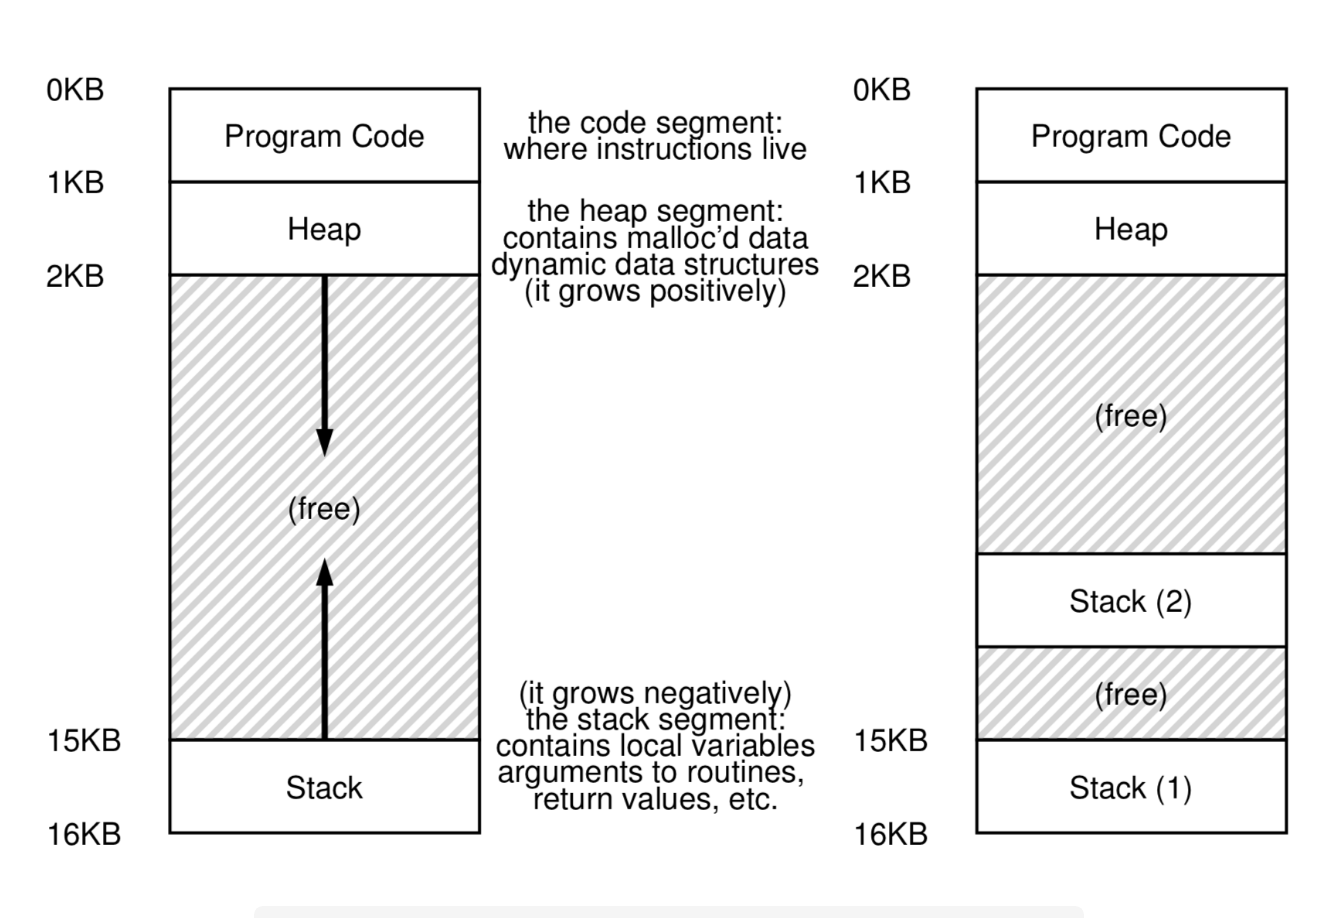
\includegraphics[width=0.65\textwidth]{chapters/Cucurrency/Cucurrency/ThreadAddressSpace.png}

\ssc{Benefit of using threads}

\sssc{Parallelism}

    Run works parallelly.

\sssc{Avoid Blocking}

    Avoid blocking program progress due to slow I/O; while one thread
    in the program waits, the CPU scheduler can switch to other ready threads.

    Threading enables overlap of I/O with other activities within a single program.

\sssc{Why not use processes instead?}

    Threads make it easy to share data, and often used to corporate with other threads
    to finish tasks.

    Processes are more sound choice for logically seperate tasks when little sharing
    of data structures in memory is needed.


\ssc{Problem with threads: Race Condition}

    \tbi{The execution sequence of threads is indeterministic}.

    Create two threads to update on the same global variable with the same function.
    
    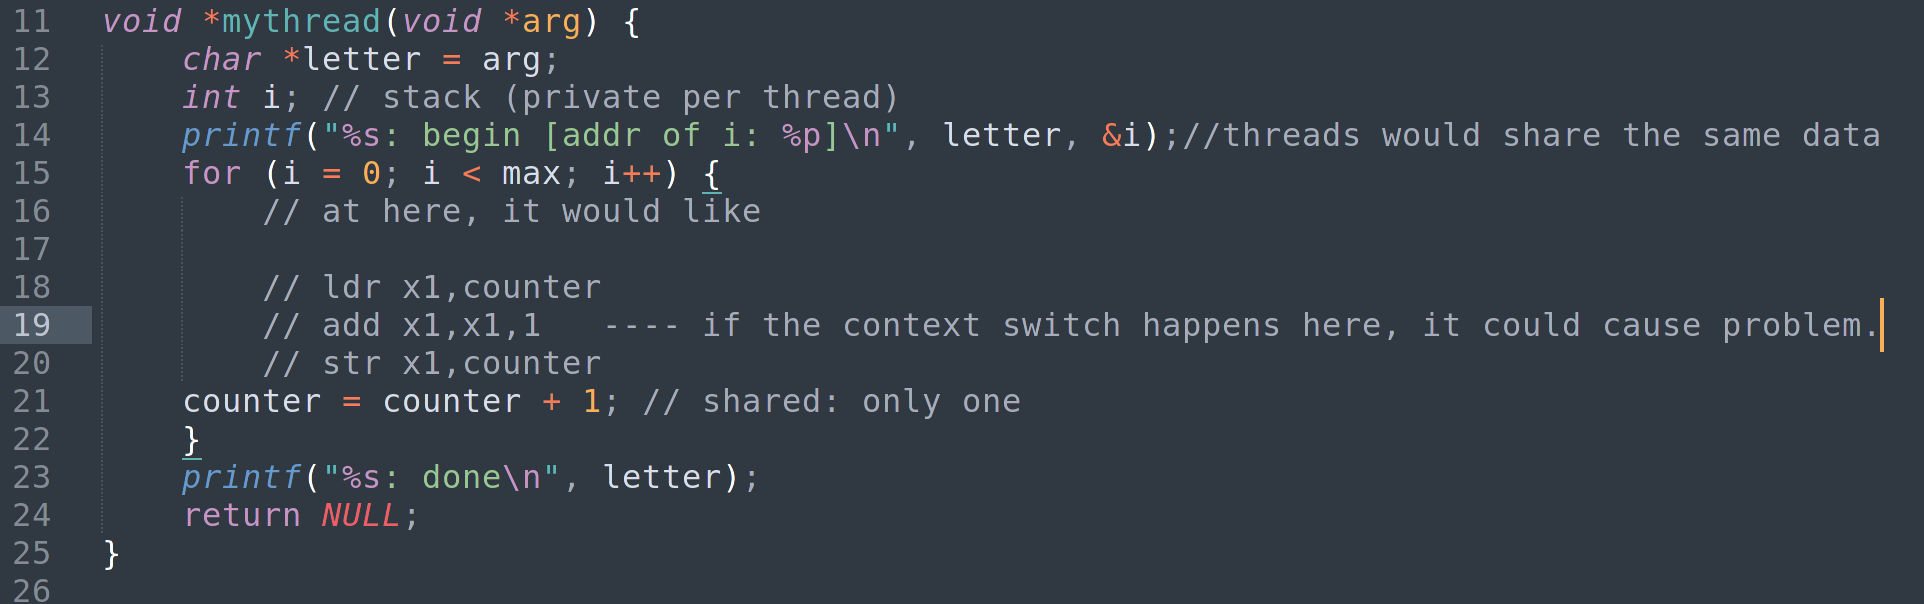
\includegraphics[width=0.75\textwidth]{chapters/Cucurrency/Cucurrency/thread_function.png}

    The problem can be:

    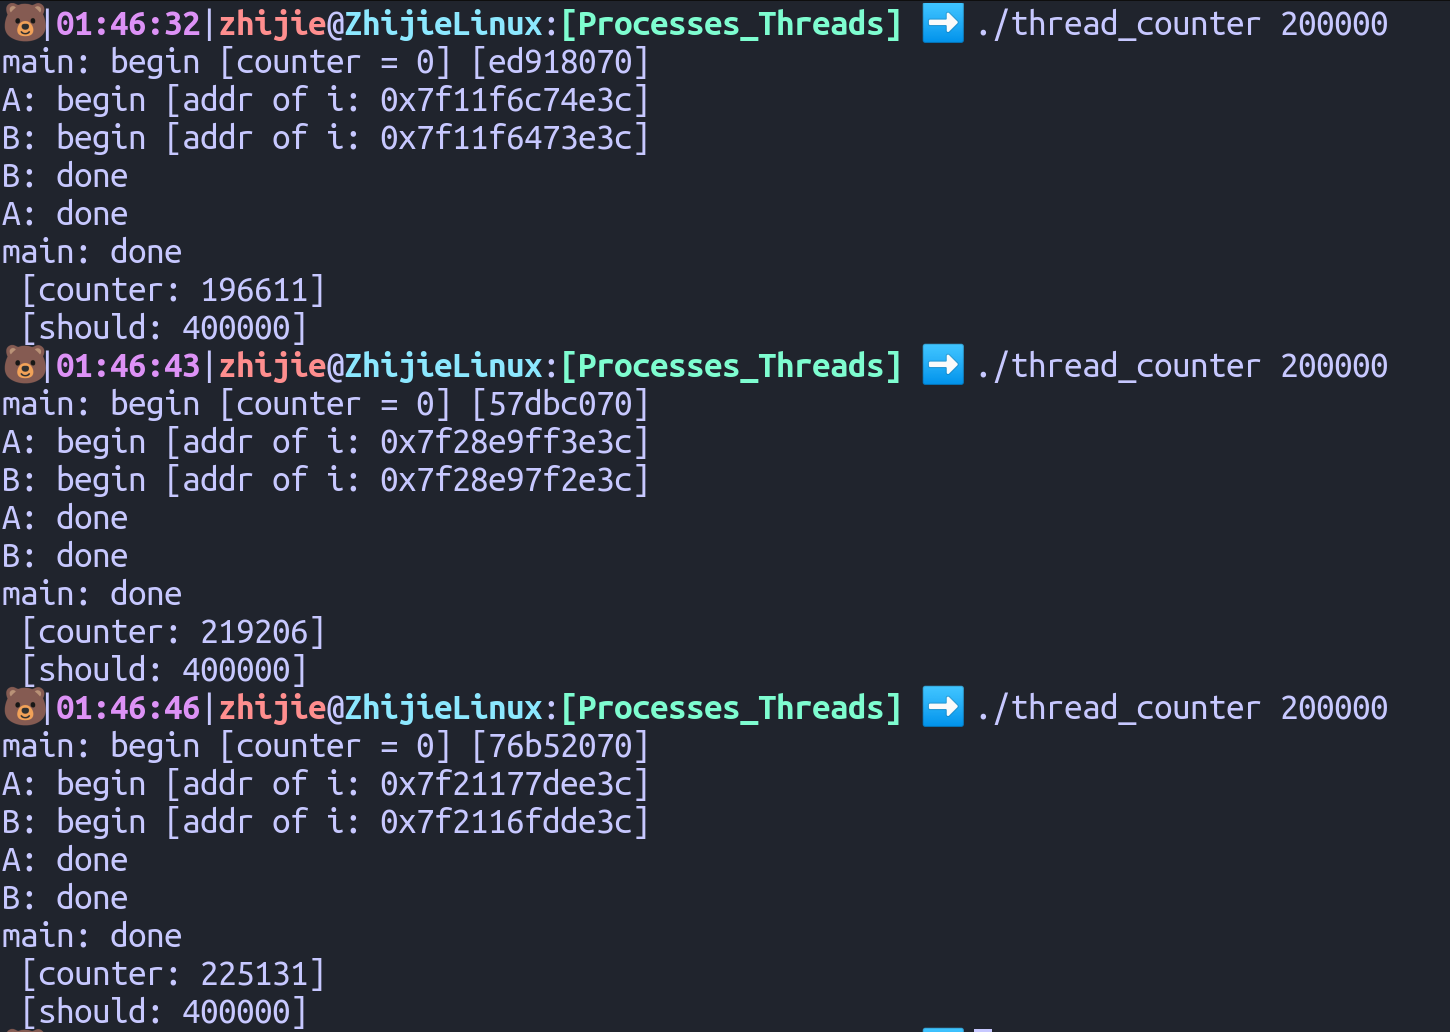
\includegraphics[width=0.7\textwidth]{chapters/Cucurrency/Cucurrency/thread_conflicts.png}


\sssc{Assembly Code}

    In ARMx8 Assembly:

    counter = counter + 1 is equivalent to 
    \begin{enumerate}
        \item ldr x1,[counter]
        \item add x1, x1, 1
        \item str x1, [counter]
    \end{enumerate}

\sssc{The work flow of causing problem}

    \begin{enumerate}
        \item Thread A loads counter into x1, say x1=50.
        \item Context switch happenes, and switch to Thread B.
        \item Now thread B loads counter into x1, x1=50.
        \item Thread B increase x1 by 1, x1=51.
        \item Thread B stores x1 back to counter, counter=51.
        \item Context switch happenes, and switch back to Thread A.
        \item Context Switch restores x1 for A,i.e, x1=50. And A won't load counter to x1 again
        \item Thread A increase x1 by 1, x1=51.
        \item Thread A stores x1 back to counter, counter=51.
        \item Thus, counter is set to 51 twice, although it should be 52 after the flow.
    \end{enumerate}

\sssc{Critical Section}

   \tbi{Critical Section}: A piece of code that accesses a shared variable, and
   must not be concurrenctly executed by more than one thread.
   
\sssc{Mutual Exclusion}

    \tbi{Mutual Exclusion:} if one thread is executing within the critical section, 
    the others will be prevented from doing so.

\sssc{Race Condition}

    Multiple threads of execution enter the critical section at roughly the same
    time; both attempt to update the shared data structure, 
    leading unexpected outcome.

\sssc{Atomicity}

    Atomic operation: grouped actions to be executed in one scheduling, i.e,
    the operation won't be interrupted.

    For example, x1 = x1 + x2 could be done in one single step with hardware support,
    instead of load, add, and store.

    It is desired to support atomicity for critical sections.   



\ssc{Thread API}

\sssc{Lock}
     
    In POSIX library, a lock needs to be initialized

    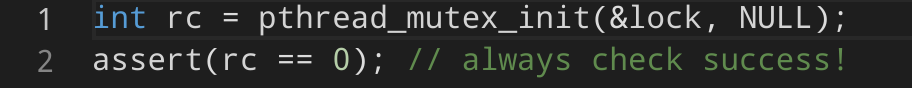
\includegraphics[width=0.6\textwidth]{chapters/Cucurrency/Cucurrency/init_lock.png}

    Also, a thread can acquire a lock, and release a lock.

    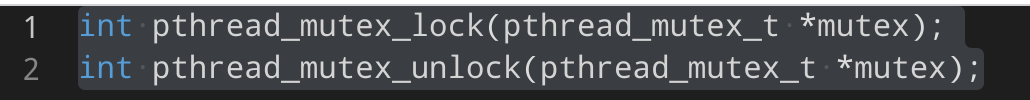
\includegraphics[width=0.6\textwidth]{chapters/Cucurrency/Cucurrency/lock_unlock.png}


\sssc{Condition Variable}

    Condition variables are useful when some kind of signaling must take place
    between threads if one thread is waiting for another to do something before it 
    continues.

    
\includegraphics[width=0.6\textwidth]{chapters/Cucurrency/Cucurrency/condtion_wait_signal.png}

    A thread must hold a lock to call either wait() or signal(). 
    $pthread_cond_wait()$, puts the calling thread to sleep.
    $pthread_cond_signal()$ awakes the waiting thread.

    The reason that $pthread_cond_wait()$ takes two parameter is because
    it needs to specify which thread to give the lock to. When $pthread_cond_wait()$
    the calling thread release the lock and pass it to another thread.

\ssc{Locks}

